\documentclass[draft]{phd}

\begin{document}
	%
	\chapter*{Introduction}
	%
		%
		Nowadays, in the most agreed picture of the nature, physicists believe in the existence of four fundamental forces, gravitational, electromagnetic, strong nuclear and weak nuclear. 
		The main open problem in theoretical physics in the last half century is certainly the description of the four fundamental forces in a single unified framework.
		So far we have witnessed impressive progresses for the last three interactions. 
		We have a theory that describes them in quite a satisfactory way, even if several points remain obscure. 
		This theory makes use of the \emph{Quantum Field Theory} -- a framework where local excitations interact according to the laws of quantum mechanics and special relativity -- and is commonly known as the \emph{Standard Model}. 
		It is, as far as we know, the most complete, experimentally verifiable theory of fundamental interactions. 
		Currently, the Standard Model is the agreed picture of fundamental physics among the physicists, also thanks to the important results from \textsc{CERN} and from many other laboratories. 
		It has the important property of being \emph{renormalisable}. 
		Indeed, some infinite quantities appear in calculating, for instance, correlators with perturbative methods. 
		This problem afflicted many of the most brilliant minds of the last century, since correlation functions are related to observable quantities, that, of course, cannot be divergent. 
		\emph{Renormalisation} is the procedure that removes these divergencies.
		
		In what follows, we will focus on the so-called ultraviolet divergencies, since these are the relevant ones for the present discussion.
		Usually in a quantum field theory, these divergencies may exist, but it is possible to introduce a finite set of, sometimes called, \emph{regularisation parameters}, such that physical quantities end up being finite. 
		Then, renormalisation consists in the redefinition of the ``constants'' of the theory (mass, charge, etc.) through this set in such a way that the finite result is set-independent.
		Obviously, there is a problem in this approach: it is not always applicable.
		There are several conditions a theory must satisfy in order to be renormalisable, and Einstein's general relativity, the currently accepted theory of gravity, is not, furthermore there is not a full satisfactory description of gravity in terms of quantum field theory.
 
		The incompatibility of general relativity and quantum field theory is not only unsatisfactory from a theoretical perspective, but hampers the construction of a consistent theory of quantum gravity and the understanding of black holes.
		Several extensions of Standard Model and brand new frameworks have been proposed in order to incorporate gravity into a quantum field description, but none of them can be confirmed by experiments yet. 
		However, among the candidates for a quantum theory of gravity, string theory is perhaps the most promising one. 
		It is based on the simple but revolutionary idea of replacing, at the fundamental scale, point-like particles with one-dimensional extended objects -- the strings.
		This simple idea has a lot of very deep and still not completely understood and discovered implications, but the theory seems to be able to unify all forces of nature.
			%
				\begin{figure}[h]
					\centering
						\scalebox{.3}{\includegraphics{./Resources/Images/Stringtheory.jpg}}
				\end{figure}
			%
			
		According to string theory, the fundamental constituents of the universe are extremely tiny vibrating strings moving in spacetime.
		These objects can appear in two different topologies, the segment and the circle, \emph{i.e.} we can have open and closed strings.
		For each of these topologies, the quantised string has a discrete spectrum of vibrating modes, which at large distances (much larger than the characteristic string length $\ell_s = \sqrt{\alpha'}$) can be effectively
interpreted as different point particles.
		The spectrum of these modes is formed by an infinite tower of states, whose lowest-lying ones are massless, while the upper levels are massive, with a spacing of $1/\sqrt{\alpha'}$.
		The theory was invented in another context (to describe strong interactions), but it came back to glory when it was realised that in the spectrum of the closed string there is always a massless spin 2 mode.
		One can identify it with the graviton, then string theory automatically incorporates gravity.
		The short distance singularities are avoided by imposing a finite length for the string.
		As a matter of fact, substituting point particles with extended objects, we get a world-sheet that is a smooth manifold and the interaction vertices are given by diagrams as in~\cref{stringdiagram}.
			%
				\begin{figure}[ht]
					\centering
						\scalebox{1.3}{\documentclass[border=5mm,tikz]{standalone}

\usepackage{amsmath, amssymb, amsfonts, amscd, amsthm, bigints, units}
%!TEX encoding = UTF-8 Unicode
\usepackage{tikz}
\usepackage{tikz-cd}
\usepackage{tikz3dcs-pp}
\usepackage{pgfplots}
\usepackage{xcolor, eecolors}
\usepackage{math, lrmath}

\usepackage{pgfplots}
\usepgfplotslibrary{patchplots}
\pgfplotsset{compat=1.15}

\usetikzlibrary{calc, intersections}

\usetikzlibrary{decorations.pathmorphing,calc,shapes,positioning,fit,arrows,fadings,decorations.pathreplacing,decorations.pathmorphing,intersections,patterns, trees}
\usetikzlibrary{decorations.markings}

\usepackage{marvosym}

%%%%%%%%My Tikz definitions%%%%%%%%%%%%%%%%%
\tikzset{->-/.style={decoration={
  markings,
  mark=at position #1 with {\arrow{latex}}},postaction={decorate}}}
  %
\tikzset{
    %Define standard arrow tip
    >=stealth',
    %Define style for boxes
    punkt/.style={
           rectangle,
           rounded corners,
           draw=black, very thick,
           text width=7.5em,
           minimum height=2em,
           text centered},
    % Define arrow style
    pil/.style={
           ->,
           thick,
           shorten <=2pt,
           shorten >=2pt,}
}
%%%
%%3d drawings %%%
\newcommand\pgfmathsinandcos[3]{%
  \pgfmathsetmacro#1{sin(#3)}%
  \pgfmathsetmacro#2{cos(#3)}%
}
\newcommand\LongitudePlane[3][current plane]{%
  \pgfmathsinandcos\sinEl\cosEl{#2} % elevation
  \pgfmathsinandcos\sint\cost{#3} % azimuth
  \tikzset{#1/.style={cm={\cost,\sint*\sinEl,0,\cosEl,(0,0)}}}
}
\newcommand\LatitudePlane[3][current plane]{%
  \pgfmathsinandcos\sinEl\cosEl{#2} % elevation
  \pgfmathsinandcos\sint\cost{#3} % latitude
  \pgfmathsetmacro\yshift{\cosEl*\sint}
  \tikzset{#1/.style={cm={\cost,0,0,\cost*\sinEl,(0,\yshift)}}} %
}
\newcommand\DrawLongitudeCircle[2][1]{
  \LongitudePlane{\angEl}{#2}
  \tikzset{current plane/.prefix style={scale=#1}}
   % angle of "visibility"
  \pgfmathsetmacro\angVis{atan(sin(#2)*cos(\angEl)/sin(\angEl))} %
  \draw[current plane] (\angVis:1) arc (\angVis:\angVis+180:1);
  \draw[current plane,dashed] (\angVis-180:1) arc (\angVis-180:\angVis:1);
}
\newcommand\DrawLatitudeCircle[2][1]{
  \LatitudePlane{\angEl}{#2}
  \tikzset{current plane/.prefix style={scale=#1}}
  \pgfmathsetmacro\sinVis{sin(#2)/cos(#2)*sin(\angEl)/cos(\angEl)}
  % angle of "visibility"
  \pgfmathsetmacro\angVis{asin(min(1,max(\sinVis,-1)))}
  \draw[current plane] (\angVis:1) arc (\angVis:-\angVis-180:1);
  \draw[current plane,dashed] (180-\angVis:1) arc (180-\angVis:\angVis:1);
}
%%%%


\begin{document}

	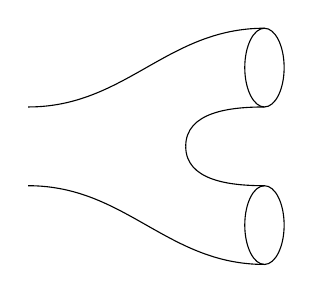
\begin{tikzpicture}[rotate=90]
		  \def\R{0.5}
		  \def\angEl{-30}
			   \DrawLatitudeCircle[\R]{0}
			  %\draw[dashed] (0,.5) arc (0:180: .5 and .25);
			  %\draw (0,.5) arc (180:360: .5 and .25);
			  \draw (-1,-3) ellipse (.5 and .25);
			  \draw (1,-3) ellipse (.5 and .25);
			  \draw (-.5,0) to[out=-90,in=90] (-1.5,-3);
			  \draw (.5,0) to[out=-90,in=90] (1.5,-3);
			  \draw (-.5,-3) to[out=90,in=180] (0,-2);
			  \draw (0,-2) to[out=0,in=90] (.5,-3);
	\end{tikzpicture}

\end{document}
}
					\caption{Feynman diagram of a string interaction vertex. 
						Imposing the finite dimension of the fundamental objects, we lose the \emph{locality} of the interactions, but we can cure the short-distance divergences.
						Now, Feynman diagrams are smooth $2$-dimensional surfaces and the interaction vertices have been ``smoothed out''.
					 }
					\label{stringdiagram}
				\end{figure}
			%
		This provides an ultraviolet regularisation of the graviton scattering amplitudes, whose divergence was due to the point-wise nature of the interaction.
		
		From a formal point of view, the only parameter in the theory that is needed to be measured is $\alpha'$, connected to the string length.
		The quantisation of the string motion imposes further constraints, \emph{e.g.} the spectrum of the bosonic string\footnote{%
			A string theory where only bosonic modes are allowed.}
		contains tachyons, which can be interpreted as instabilities of the space-time.
		This can be avoided by introducing supersymmetry, giving rise to \emph{superstring theory}.
		Historically, the introduction of supersymmetry and the developing of superstring theory is called \emph{first string revolution}.
		
		From the point of view of an observer that sits on the string, string theory can be seen as a two-dimensional field theory (\emph{i.e.} the field theory on the two-dimensional string world-sheet).
		This theory turns out to have a complete conformal symmetry.
		We want to preserve this world-sheet symmetry even after the quantisation procedure. The conditions to have Weyl anomaly\footnote{%
			An \emph{anomaly} is a quantum effect breaking a classical symmetry. The Weyl anomaly is the anomaly breaking the conformal symmetry.}
		cancellation constrain the space-time to be ten-dimensional.
		Taking into account all the constraints and consistency conditions, it turns out that there are only five possible superstring theories: type I, type IIA, type IIB and the two heterotic theories $\SO(32)$ and $\E_8 \times \E_8$.
		In mid 1990s the concept of dualities arose in string theory, giving start to a process called \emph{second string revolution}, and this allowed to discover that superstring theories are actually different formulations of the same theory.
		Indeed, all these formulations are connected by a net of dualities, that involve other fundamental dynamical objects, further than strings, called branes.
		These interconnections among the different superstring theories might be the signal of an underlying more fundamental theory, which is conjectured to live in eleven spacetime dimensions, and has been given the name of M-theory\footnote{%
			We know the $11$-dimensional supergravity, so the corresponding high energy fundamental theory is identified with M-theory.
			We do not have a complete formulation of M-theory yet, but we know the degrees of freedom of the theory.
			This tells us that the fundamental dynamical ingredients of this theory are not strings, but higher dimensional objects: branes.
			We are going back to branes in the following.}.		
		
		As mentioned above, at low energies strings might be considered as particles. 
		The theory coming out of the particle limit of string theory is \emph{supergravity}.
		As the name may suggest, \emph{supergravity} is a theory encoding both Einstein gravity and supersymmetry (making this a point-wise symmetry).
		It was discovered independently from string theory in mid seventies, and only at a later stage physicists realised it was a limit at low energy scales of the latter.
		
		The introduction of finite dimensional elementary objects seems to solve the conflict between general relativity and quantum field theory. 
		In addition, since it also seems to contain gauge bosons, it provides a framework for the unification of all fundamental forces, that reproduces, as low energy limit, Einstein’s theory and gauge theories.
		However, we pay a price. Space-time has extra-dimensions.
		This is one of the most striking predictions of string theory, and a model based on this framework with some hope to describe nature has to cope with this issue.
		
		One option to face this concern is to find a way to reduce the space-time dimension: from $10$ or $11$ dimensional down to $4$.
		The most common way to achieve this reduction is through a procedure called \emph{compacification}.
		It consists in assuming the original spacetime to have only four spacetime directions -- the ones we have experience of -- and the remaining ones are instead wrapped on themselves to form a compact space.
		The characteristic dimension of this space is very small, such to explain why we do not have access to it (there are actually some bounds on the maximal length these dimensions can have. These bounds are being updated constantly due to on going measures at LHC, see for example~\cite{extradim1,extradim2}).
		More formally, we take into account spacetime solutions with a topology like,
			%
				\begin{equation*}
					\mathcal{M}_D \rightarrow \mathcal{X} \times M_d\, ,
				\end{equation*}
			%
		where $\mathcal{X}$ is called \emph{external spacetime}, and $M_d$ is the compact \emph{internal} manifold.
		In order to get an effective field theory in lower dimension, one has to integrate the higher dimensional theory over the internal manifold to get only external spacetime quantities.
		
		The features of the effective lower dimensional theory depends in a dramatic way from the geometry of the internal space.
		One of the most important constraints we want to introduce is the amount of supersymmetry preserved in the compactification.
		From a phenomenological point of view, the most desirable case is preserving a minimal amount of supersymmetry, since the minimal extensions of the Standard Model requires minimal supersymmetry\footnote{%
			We want to make contact with supersymmetric extensions of Standard Model because the scale of supersymmetry breaking in these models is usually much lower than the compactification scale.}.
		The non-complete breaking of supersymmetry is welcome also for technical purposes, since -- according to the common idea ``more symmetry, more constraints'' -- it allows for more control on the compactified theory.
		Supersymmetry conditions translate into topological and differential conditions on spinors of the internal manifold, and this strongly constrains the geometry.
		In a very famous example, a ten-dimensional supergravity is compactified to a minimal ($\mathcal{N}=1$) supergravity theory in $4$-dimensions. Taking a vacuum as reference, \emph{i.e.} the effective field theory will be the study of fluctuations about this vacuum, where all the internal supergravity fields except the metric are set to zero, the compactification manifold is required to be a Calabi-Yau three-fold, namely a $6$-dimensional manifold with $\SU(3)$ holonomy~\cite{CYcomp}.
		This is a very popular result, however, it turns out that the number of possible Calabi-Yau manifolds is finite, but huge\footnote{%
			The order of magnitude is $10^{500}$.}. 
		Hence, the choice of the supersymmetric background is not unique at all.
		
		Reasons to study compactifications are not only phenomenological.
		There are important formal motivations.
		Many supergravity theories in various dimensions are connected by compactifications.
		Historically, since the birth of supergravity, dimensional reductions have been used to build lower dimensional models from the higher dimensional ones, since the spectrum of the latter is usually simpler.
		A first milestone example is the derivation of the four-dimensional maximally supersymmetric supergravity theory from the eleven-dimensional supergravity, due to Cremmer and Julia~\cite{CremmerJulia}.
		
		We will see that the modern approach to model building via compactifications involves several ingredients. 
		Among these there are localised objects like D- or M-branes, which typically are taken intersecting among them.
		For various reasons, one is also led to add other tools like fluxes of the higher-dimensional fields and non-perturbative quantum effects. 
		Clearly, it is very hard to have full control on all these ingredients at once, so that often one prefers to focus on certain aspects of the whole picture. 
		In this thesis, we will focus on the relation between geometry and supersymmetry in compactifications, having a look also at supersymmetric conditions for branes.
		
		We are going to expose some facts about compactifications and geometry.
		Further, we collect some notions about branes and their supersymmetric configurations, since this will be the matter of~\ref{chapbrane}. 
		%
	\subsection*{Compactifications and fluxes}
		%
			The idea of introducing extra-dimension to get some sort of unification of different phenomena is not recent.
			It dates back to the works of Kaluza and Klein~\cite{Kaluza, Klein} who studied a purely gravity theory in five dimensions in order to incorporate the Maxwell's electromagnetism into Einstein's gravity.
			The idea is to add a $4$-th spatial dimension and then to operate a dimensional reduction. In this way one recovers the effective field theory of electromagnetism coupled to gravity on the usual $4$-dimensional spacetime.
			Nowadays, we indicate as \emph{Kaluza-Klein dimensional reduction} generically the compactification on a $n$-circle.
			
			We want to briefly review the Kaluza-Klein reduction in arbitrary dimension.
			We will follow~\cite{stellereview, popeKK}.
			Firstly, we aim to reduce a $(d+1)$-dimensional purely gravitational theory down to $d$-dimensions, by a reduction on a circle $S^1_R$ of radius $R$.
			For simplicity, we suppose the $d$-th spatial coordinate is the periodic one, and we call it $y$, \emph{i.e.} for any integer $k$, $y + 2\pi k R \simeq y$.
			The $(d+1)$-dimensional vector of coordinate is $z^M \equiv (x^\mu , y)$, where $M = 0,\ldots, d$ and $\mu = 0, \ldots d-1$.
			
			Let us take into account the usual Einstein-Hilbert action for $(d+1)$-dimensional gravity,
				%
					\begin{equation*}
						\mathcal{S} = \frac{1}{2 \mathrm{k}^2} \int \dd^{d+1}z\ \sqrt{-\mathfrak{g}}\ \mathcal{R} \, .
					\end{equation*}
				%
			The periodicity of the $d$-th spatial dimension allows us to write the expansion in Fourier modes of the metric along that direction
				%
					\begin{equation*}
						\mathfrak{g} (x, y) = \sum_{k} g^{(k)}(x) e^{i k y / R} \, .
					\end{equation*}
				%
			At this point we can substitute the Fourier expansion in the action and integrate $y$ away over the $S^1$.
			However, doing this one would have a $d$-dimensional theory with an infinite tower of states, labeled by $k$.
			In order to find an effective lower dimensional theory with a finite number of degrees of freedom, we have to define a so-called \emph{truncation ansatz}, namely a prescription telling us which modes (in this case of the metric expansion) we keep and which ones are to set to zero.
			In this toy-model the criterium to truncate the spectrum is readable by the equation of motion (the Einstein equation $\mathcal{R}_{MN} = 0$).
			Precisely, linearising this for small fluctuations around the flat Minkowski solution $\mathbb{M}_{d} \times S^1$, we get
				%
					\begin{equation*}
						\langle \mathfrak{g}_{MN} \rangle \dd z^M \dd z^N = \eta_{\mu\nu} \dd x^\mu \dd x^\nu + \dd y^2 \, , 
					\end{equation*}
				%
			where we assumed the v.e.v. of the last component to be $\langle \mathfrak{g}_{dd} \rangle = 1$.
			Taking the circle radius $R$ small enough, we can make all the states with $n\neq 0$ very massive, thus we can neglect them in a low energy approximation of the theory.
			To conclude, we can define a truncation to lower dimensional massless modes by keeping all the $d+1$-dimensional fields that are $y$-independent.
			For instance, we can reduce the higher dimensional metric as follows,
				%
					\begin{equation*}
						\mathfrak{g}_{MN} \dd z^M \dd z^N =  e^{2\alpha \phi(x)} g_{\mu\nu} \dd x^\mu \dd x^\nu + e^{2\beta \phi(x)} (\dd y + A )^2\, ,
					\end{equation*}
				%
			where $\alpha$ and $\beta$ are real parameters and $\phi(x)$ is a real function of the $x$ coordinates only. 
			Lastly, $A$ is a one form $A_{\mu}(x) \dd x^\mu$.
			Explicitly, this ansatz gives the prescriptions,
				%
					\begin{align*}
						&& \mathfrak{g}_{\mu\nu} = e^{2\alpha \phi} g_{\mu\nu} + e^{2\beta \phi} A_{\mu} A_{\nu} \, , && \mathfrak{g}_{\mu d} = e^{2\beta \phi} A_{\mu} \, , & & \mathfrak{g}_{dd} = e^{2\beta\phi} \, . & &
					\end{align*}
				%
			
			Substituting the quantities in the higher dimensional action functional, and integrating over $S^1$, allows us to write
				%
					\begin{equation*}
						S = \frac{1}{2 \kappa^2} \int \dd^{d}x\ \sqrt{-g}\ \left(R - \frac{1}{2} (\partial \phi)^2 - \frac{1}{4} e^{-2(d-1) \alpha \phi} F_{\mu\nu}F^{\mu\nu} \right)\, ,
					\end{equation*}
				%
			where $F_{\mu\nu} = 2 \partial_{[\mu} A_{\nu]}$ and $\kappa^2 = \mathrm{k}^2/ 2\pi R$.
			We imposed also a the following normalisations for $\alpha$ and $\beta$,
				%
					\begin{align*}
						&& \alpha^2  = \frac{1}{2(d-2)(d-3)} \, , & & \beta = - (d-3) \alpha \, ,& &
					\end{align*}
				%
			in order to get a correctly normalised kinetic term for the scalar field~\cite{popeKK}.
			
			To conclude, we obtained the Maxwell-Einstein action -- with an additional scalar $\phi$ called \emph{modulus}, on which we will come back shortly -- by reducing a purely gravitational theory on a circle.
			The gauge symmetry $A \rightarrow A + \dd \lambda$ is a consequence of the metric ansatz, when one ($x$-dependently) reparametrises the circle.
			
			The reduction exposed above is a useful toy-model of reduction.
			However, in string and supergravity compactifications one has to cope with much more involved techniques.
			This because the action is not just gravity and also because the compactification manifold is usually more complicated than a circle.
			Despite this, there are some main points we can highlight since they are common to a large number of compactification procedures.
			
			As previously mentioned, we want a lower dimensional theory with a finite number of degrees of freedom.
			In order to achieve this, we have to give a prescription indicating which fields we keep and which ones we have to ``truncate out''.
			In other words a truncation of the higher dimensional modes on the internal manifold is necessary.
			We call this prescription \emph{truncation ansatz}.
			In our toy-example, the truncation ansatz was readable explicitly, but in general life is much harder.
			
			One way to procede is to focus on a vacuum state in low dimension and study the perturbations about this vacuum.
			The truncation prescription is given by the so-called \emph{Kaluza-Klein ansatz}.
			A nice review about this topic is given in~\cite{duffKK}.
			
			Briefly speaking, the procedure to get the truncation ansatz can be described schematically as follows.
			Firstly, one considers a vacuum of the higher dimensional theory that exhibits a spacetime solution structure as a product of spaces, the lower-dimensional spacetime and the internal space.
			Secondly, the equations of motion are linearised around vacuum.
			This produces some massive operators from the lower-dimensional perspective.
			Expanding the higher-dimensional degrees of freedom into the eigenstates of these massive operators, and keeping only the massless modes concludes the procedure.
			
			It is noteworthy that in general the ansatz gives a good way to study linear fluctuations about the chosen vacuum, but the theory coming out of this might not capture the whole information the higher-dimensional theory had originally.
			In the previous example the expansion to all-order of the ansatz was achieved by truncating out all the fields depending on the coordinate on the circle.
			However, already taking into account slightly more complicated spaces this extension will be highly non-trivial, often not possible at all.
			Therefore, Kaluza-Klein anstaze are limited to describe the physics around a chosen vacuum.
			
			One can chose to follow another approach.
			This consists of defining a truncation ansatz based on a given symmetry, that is keeping the modes which are invariant under some group of transformations.
			The typical group of transformations one takes into account is a subgroup of the isometry group of the internal manifold.
			This approach can be applied with fruitful results to the cases where the internal manifold is a group manifold or a coset space, since the isometry group is manifest~\cite{Cvetic:2003jy, schschw}.
			The simplest example to consider is the $\U(1)$ reduction.
			Notice that since $S^1 \cong \U(1)$, our toy example describes this second approach as well.
			Keeping only the higher dimensional fields independent on $y$ is equivalent to take only the invariant fields (\emph{i.e.} the singlets) under the $\U(1)$ action.
			
			At this stage, it is useful to make some remark about this second approach.
			A first point to raise, the truncated theory is not always physically relevant, since the lower dimensional physics may not be captured completely by the compactified theory.
			However, it is mathematically well-defined and independent from the choice of a specific vacuum.
			The second noteworthy aspect -- crucially important in this thesis -- is that the dimensional reduction based on the use of a symmetry is able to give ansatze that are \emph{consistent}.
			A \emph{consistent truncation} is a choice of a finite set of modes, where the omitted ones are not sourced by the subset chosen. 
			This is equivalent to say that the set of truncated modes has a dynamics which is not affected by the others.
			This fact allows us to say that a solution to equations of motion in the lower dimensional theory, which is a linear combination of only truncated modes, always lift to a solution also on the higher dimensional theory.
			It might be useful to consider a simple example to understand what we mean for consistent truncations.
			Given a theory of two scalars with Lagrangian,
				%
					\begin{equation*}
						\mathcal{L} = \frac{1}{2}\left(\partial \varphi_1 \right)^2 + \frac{1}{2}\left(\partial \varphi_2 \right)^2 - \frac{m_1^2}{2}\varphi_1^2 - \frac{m_2^2}{2}\varphi_2^2 - g \varphi_1^2\varphi_2 \, .
					\end{equation*}
				%
			It generates the following equations of motion,
				%
					\begin{equation*}
						\begin{split}
							\partial_\mu \partial^\mu \varphi_1 + m_1^2 \varphi_1 &= -2g\varphi_1\varphi_2 \, , \\
							\partial_\mu \partial^\mu \varphi_2 + m_2^2 \varphi_2 &= -g\varphi_1^2 \, .
						\end{split}
					\end{equation*}
				%
			Therefore, we can observe how $\varphi_1 = 0$ is a consistent truncation, \emph{i.e.} the evolution of $\varphi_2$ is given by a consistent (with the choice of suppressing $\varphi_1$) equation of motion, and fixed $\varphi_1 = 0$ at the initial time, it will remain fixed at all times. 
			In other words, $\varphi_1 = 0$ is both a solution of the theory reduced to the only field $\varphi_1$, and of the full theory of the two scalar fields $\varphi_1,\varphi_2$. 
			On the other hand, dropping $\varphi_2 = 0$ is not consistent, since the dynamics of $\varphi_1$ will affect $\varphi_2$, due to the fact $\varphi_1$ acts as a source term for $\varphi_2$.
			
			In this very simple example, the truncation it is easy to find by simply playing with the equations of motion.
			Not surprisingly, in the case of dimensional reductions things are not so simple and in order to have the hope of finding a consistent truncation we have to rely on symmetry.
			
			Let us reconsider our toy-model of reduction again.
			We have seen how by dimensionally reducing a theory of gravity over a circle we get a theory of gravity coupled with electromagnetism and a free massless scalar (at linear order). 
			This field is related to the radius of the compactification circle and how it varies along the $d$-dimensional spacetime.
			There is not a procedure that tells us which value $R$ has to take dynamically during the compactification and this reflects in the presence a free scalar, \emph{i.e.} with no fixed (by some potential) \emph{vacuum expectation value}, vev from now on.
			This is a characteristics that is often present in compactifications: the background exhibits a continuous degeneracy related to the variations in size and shape of the compact space.
			The fields parametrising this degeneracy are called \emph{moduli} and when the compactification does not produce any scalar potential (which constrains their vevs), one says moduli are not \emph{stabilised}.
			In our example we just have one massless scalar field, but typically Calabi-Yau compactifications produce a large number of moduli.
			This goes under the name of \emph{moduli problem}.
			
			One wants moduli to be stabilised for various reasons.
			First of all, the observables of the lower-dimensional theory depends on the moduli, so, if their vevs can be shifted arbitrarily the theory loses predictivity.
			One may be thinking that this situation is similar to handle Goldstone bosons.
			Spontaneous symmetry breaking is the reason of the origin of the Goldstone modes, indeed the physics in any vacuum connected by a Goldstone mode is the same, since all these vacua are equivalent due to symmetry.
			Moduli, however, do not need a symmetry to arise and hence in general physics will depend on their values.
			Then one finds a space of physically inequivalent vacua (the notorious \emph{moduli space}) related by varying the vev of the moduli.
			Furthermore, phenomenologically massless scalar fields should mediate long range interactions, but this contradicts the observations.
			Finally, a more formal point of view is to answer to the question ``how can the masses of particles in Standard Model come from a theory with no free parameters?''~\cite{moduliLect, fluxcomp1}.
				
				%
					\begin{figure}[h!]
						\centering
						\documentclass[border=5mm,tikz]{standalone}

\usepackage{amsmath, amssymb, amsfonts, amscd, amsthm, bigints, units}
%!TEX encoding = UTF-8 Unicode
\usepackage{tikz}
\usepackage{tikz-cd}
\usepackage{tikz3dcs-pp}
\usepackage{pgfplots}
\usepackage{xcolor, eecolors}
\usepackage{math, lrmath}

\usepackage{pgfplots}
\usepgfplotslibrary{patchplots}
\pgfplotsset{compat=1.15}

\usetikzlibrary{calc, intersections}

\usetikzlibrary{decorations.pathmorphing,calc,shapes,positioning,fit,arrows,fadings,decorations.pathreplacing,decorations.pathmorphing,intersections,patterns, trees}
\usetikzlibrary{decorations.markings}

\usepackage{marvosym}

%%%%%%%%My Tikz definitions%%%%%%%%%%%%%%%%%
\tikzset{->-/.style={decoration={
  markings,
  mark=at position #1 with {\arrow{latex}}},postaction={decorate}}}
  %
\tikzset{
    %Define standard arrow tip
    >=stealth',
    %Define style for boxes
    punkt/.style={
           rectangle,
           rounded corners,
           draw=black, very thick,
           text width=7.5em,
           minimum height=2em,
           text centered},
    % Define arrow style
    pil/.style={
           ->,
           thick,
           shorten <=2pt,
           shorten >=2pt,}
}
%%%
%%3d drawings %%%
\newcommand\pgfmathsinandcos[3]{%
  \pgfmathsetmacro#1{sin(#3)}%
  \pgfmathsetmacro#2{cos(#3)}%
}
\newcommand\LongitudePlane[3][current plane]{%
  \pgfmathsinandcos\sinEl\cosEl{#2} % elevation
  \pgfmathsinandcos\sint\cost{#3} % azimuth
  \tikzset{#1/.style={cm={\cost,\sint*\sinEl,0,\cosEl,(0,0)}}}
}
\newcommand\LatitudePlane[3][current plane]{%
  \pgfmathsinandcos\sinEl\cosEl{#2} % elevation
  \pgfmathsinandcos\sint\cost{#3} % latitude
  \pgfmathsetmacro\yshift{\cosEl*\sint}
  \tikzset{#1/.style={cm={\cost,0,0,\cost*\sinEl,(0,\yshift)}}} %
}
\newcommand\DrawLongitudeCircle[2][1]{
  \LongitudePlane{\angEl}{#2}
  \tikzset{current plane/.prefix style={scale=#1}}
   % angle of "visibility"
  \pgfmathsetmacro\angVis{atan(sin(#2)*cos(\angEl)/sin(\angEl))} %
  \draw[current plane] (\angVis:1) arc (\angVis:\angVis+180:1);
  \draw[current plane,dashed] (\angVis-180:1) arc (\angVis-180:\angVis:1);
}
\newcommand\DrawLatitudeCircle[2][1]{
  \LatitudePlane{\angEl}{#2}
  \tikzset{current plane/.prefix style={scale=#1}}
  \pgfmathsetmacro\sinVis{sin(#2)/cos(#2)*sin(\angEl)/cos(\angEl)}
  % angle of "visibility"
  \pgfmathsetmacro\angVis{asin(min(1,max(\sinVis,-1)))}
  \draw[current plane] (\angVis:1) arc (\angVis:-\angVis-180:1);
  \draw[current plane,dashed] (180-\angVis:1) arc (180-\angVis:\angVis:1);
}
%%%%


\begin{document}
%
	\begin{tikzpicture}
	    	
		% External Manifold
		\draw[smooth cycle, tension=0.4, fill=white, pattern color=orange, pattern=north west lines, opacity=.5] plot coordinates{(-5.7,2) (-8.2,0) (-4.7,-2) (-2.7,1)};
		\draw node at (-5, 2.3) {$\mathcal{X}$};
		\draw node at (0, 2) {$M$};
		\draw node at (-2.5,0) {$\times$};
	    
	    % \x runs over the angles at which to draw the circles defining the
	    % torus
	    \foreach \x in {90,89,...,-90} { % change 89 to 80 or 45 for speed
	    % \elrad is the x-radius of the ellipse (technically, a circle seen	
	    % from side on at angle \x).  The 'max' is because at small angles
	    % then the real ellipse is too thin and the torus doesn't ``fill
	    % out'' nicely.
	    \pgfmathsetmacro\elrad{20*max(cos(\x),.1)}
	    % We draw the torus from the back to the front to get the right
	    % layering effect.  To tint it, we define colours according to the
	    % angle, but need different colours for the left and right pieces.
	    % It'd be nice if the xcolor colour specification could take something
	    % computed by pdfmath, such as {red!\tint} but it doesn't appear to
	    % work, so we define the colours explicitly.
	    \pgfmathsetmacro\ltint{.9*abs(\x-45)/180}
	    \pgfmathsetmacro\rtint{.9*(1-abs(\x+45)/180)}
	    \definecolor{currentcolor}{rgb}{\ltint, 0, \ltint}
	    % This draws the right-hand circle.
	    \draw[color=currentcolor,fill=currentcolor] 
	        (xyz polar cs:angle=\x,y radius=.75,x radius=1.5) 
	        ellipse (\elrad pt and 20pt);
	    % This sets the colour correctly for the left-hand circle ...
	    \definecolor{currentcolor}{rgb}{\rtint, 0, \rtint}
	    % ... and draws it
	    \draw[color=currentcolor,fill=currentcolor] 
	        (xyz polar cs:angle=180-\x,radius=.75,x radius=1.5) 
	        ellipse (\elrad pt and 20pt);
	    % End of foreach statement
	    }
	   % \draw[densely dashed, yellow] (0,-1.45) arc (270:90:-.2 and .480);
		\draw[yellow, ultra thick, line cap=round] (0,-1.45) arc (-93:90:-.25 and .705);
		\draw[yellow, ultra thick, line cap=round] (-.5,-1.4) arc (-93:95:-.25 and .705);
		\draw[yellow, ultra thick, line cap=round] (-.25,-1.42) arc (-93:93:-.25 and .705);
	
	%labels
		\draw[densely dashed, thin, gray, <-] (-.5,-1.5) -- (-.7,-2.5)
			node at (-.75, -2.7) {\textcolor{black}{Fluxes}};
									
    		% Spheres are *much* easier!
%    	\shadedraw[shading=ball,ball color=purple, white] (6.5,0) circle (1.5);
%    	% As are the subsets of Euclidean space
%    	\draw[fill=cyan] (-1,-4) rectangle (1,-3);
%    	\draw[fill=cyan] (5.5,-4) rectangle (7.5,-3);
%    	% The next three draw the maps, slightly curved for aesthetics.
%    	\draw[->] (0,-2.8) .. controls (-.2,-2.2) .. (0,-1.6) 
%    	    node[pos=0.5, auto=left] {\(\psi\)};
%    	\draw[->] (6.5,-1.6) .. controls (6.7,-2.2) .. (6.5,-2.8) 
%    	    node[pos=0.5, auto=left] {\(\phi^{-1}\)};
%    	\draw[->] (2.5,0) .. controls (3.5,.2) .. (4.5,0) 
%    	    node[pos=0.5, auto=left] {\(f\)};
%    	% Now we want to draw the codomains of the charts.  Sticking cosines
%    	% and sines directly into the coordinates doesn't seem to work so
%    	% we define macros to hold the sines and cosines of the angles.
%    	% \elrad is the angle on the torus at which to start.
%    	\pgfmathsetmacro\elrad{cos(-135)}
%    	% the circle drawn at the specific angle on the torus looks like an
%    	% ellipse, \xrad and \yrad compute its major and minor semi-axes.
%    	\pgfmathsetmacro\xrad{1.5cm-20pt*\elrad}
%    	\pgfmathsetmacro\yrad{.75cm-20pt*sin(-135)}
%    	% This draws the codomain of the chart on the torus.
%    	\path[fill=cyan, fill opacity=.35] 
%    	    (xyz polar cs:angle=-135,radius=.75,x radius=1.5) 
%    	    ++(20pt*\elrad,0) arc (0:45:20*\elrad pt and 20pt) 
%    	    arc (-135:-45:\xrad pt and \yrad pt) 
%    	    arc (45:-45:-20*\elrad pt and 20pt) 
%    	    arc (-45:-135:\xrad pt and \yrad pt) 
%    	    arc (-45:0:20*\elrad pt and 20pt);
%    	% Now we do the same for the sphere.
%    	% We do this by drawing some great circles (aka ellipses) on the
%    	% sphere and then ``clipping'' an overlaid (and slightly trans:parent)
%	    % sphere by those great circles.  Each great circle actually specifies
%	    % one side of the ``clip'' so to make sure that the clip is big enough
%	    % the arcs are completed by big rectangles (otherwise the clipping
%	    % would join the end points directly).
%	    \pgfmathsetmacro\tell{-sin(10)}
%	    \pgfmathsetmacro\bell{sin(50)}
%	    \pgfmathsetmacro\rell{1.5 * sin(50)}	
%	    \begin{scope}
%	        \clip (6.5,0) +(-1.5,0) arc (-180:0:1.5 and 1.5*\tell) 
%	            -- ++(0,-1.5) -- ++(-3,0) -- ++(0,1.5);
%	        \clip (6.5,0) +(-1.5,0) arc (-180:0:1.5 and 1.5*\bell) 
%	            -- ++(0,1.5) -- ++(-3,0) -- ++(0,-1.5);
%	        \clip (6.5,0) +(0,1.5)  arc (90:-90:\rell cm and 1.5 cm) 
%	            -- ++(-1.5,0) -- ++(0,3) -- ++(1.5,0);
%	        \clip (6.5,0) +(0,1.5)  arc (90:-90:-\rell cm and 1.5 cm) 
%	            -- ++(1.5,0) -- ++(0,3) -- ++(-1.5,0);
%	        \fill[cyan, fill opacity=0.35] (6.5,0) circle (1.5);
%	    \end{scope}

	\end{tikzpicture}
	
%	\begin{tikzpicture}
%	\begin{axis}[
%      hide axis,
%      view={60}{30},
%      axis equal image,
%    ]
%    \addplot3 [
%      surf, shader=interp,
%      point meta=x,
%      colormap/greenyellow,
%      samples=40,
%      samples y=20,
%      z buffer=sort,
%      domain=0:360,
%      y domain=0:360
%    ] (
%              {(3.5 + 0.5*cos(y))*cos(x)},
%              {(3.5 + 0.5*cos(y))*sin(x)},
%              {0.5*sin(y)});
%    \addplot3 [
%     samples=40,
%     samples y=1,
%     domain=0:360,
%     thick
%    ] (
%              {(3.5 + 0.5*cos(80))*cos(x)},
%              {(3.5 + 0.5*cos(80))*sin(x)},
%              {0.5*sin(80)});
%    \addplot3 [
%      samples=10,
%      samples y=1,
%      domain=-65:130,
%      thick
%    ] (
%              {3.5 + 0.5*cos(x)},
%              {0},
%              {0.5*sin(x)});
%
%  \end{axis}
%\end{tikzpicture}

\end{document}
						\caption{A schematic representation of a compactification in the presence of fluxes.}
						\label{fluxcomp}
					\end{figure}
				%
			A possible path to follow in order to solve the moduli problem is to find a mechanism to generate a scalar potential in the lower-dimensional action.
			This would have the effect of stabilise the moduli (giving them a mass and a fixed vev).
			A great number of results in this direction have been reached in the last twenty years, realising that it is possible to generate a non-trivial scalar potential in a compactification through \emph{fluxes}~\cite{fluxcomp1, fluxcomp2, fluxcomp3}.
			One can find some nice reviews of the subject in~\cite{DuffReviewComp, MarianaFluxReview, LustReviewComp, henlect}.
			
			Fluxes are higher rank objects generalisation of the electromagnetic field strength.
			They are associated with a non-zero background value of the supergravity $p$-form field strength.
			To be precise, let $F_p$ be a $p$-form field strength whose Bianchi identity is
				%
					\begin{equation*}
						\dd F_p = 0\, ,
					\end{equation*}
				%
			locally, one can always associate a potential $C_{p-1}$ such that $F_p = \dd C_{p-1}$. 
			When sources are present it is not possible to have a globally well-defined potential, and the integral over a a $p$-cycle $\Sigma_p$ on the internal compact manifold $M$ it is not automatically zero. 
			Then we say there is a flux of $F_p$ on $M$ supported by $\Sigma_p$,
				%
					\begin{equation*}
						\frac{1}{(2\pi \ell_s)^{p-1}}\int_{\Sigma_p}\!\! F_p = k \neq 0\, .
					\end{equation*}
				%
			As for the familiar Dirac's monopole, one can impose quantisation conditions on fluxes so that $k$ can take only discrete values.
			Roughly speaking, this number corresponds to how many times the extended object associated to the flux wraps around the cycle $\Sigma_p$, see~\cref{fluxcomp}.
			Requiring the presence of these quantities in the dimensional reduction we can generate a potential $V$ for the scalars in the lower dimensional theory, that will come from the kinetic term of the internal components of  the fluxes.
			This can be seen from the higher dimensiona action. 
			Schematically,
				%
					\begin{equation*}
						S= \int_{\mathcal{X}} \ldots \underbrace{\int_{M} F \wedge \star F}_{V(\phi)} \, .
					\end{equation*}
				%
			
			Moduli stabilisation is not the only reason to study flux compactifications.
			For example, the presence of fluxes removes the necessity of a Ricci-flat internal space, then Calabi-Yau are no more available spaces.
			This open interesting perspectives in studying the geometry of string theory vacua and a classification of flux compactifications may be very useful in order to understand better the structure of the theory.
				
				%
					\begin{figure}[h!]
						\centering
						\documentclass[border=5mm,tikz]{standalone}

\usepackage{amsmath, amssymb, amsfonts, amscd, amsthm, bigints, units}
%!TEX encoding = UTF-8 Unicode
\usepackage{tikz}
\usepackage{tikz-cd}
\usepackage{tikz3dcs-pp}
\usepackage{pgfplots}
\usepackage{xcolor, eecolors}
\usepackage{math, lrmath}

\usepackage{pgfplots}
\usepgfplotslibrary{patchplots}
\pgfplotsset{compat=1.15}

\usetikzlibrary{calc, intersections}

\usetikzlibrary{decorations.pathmorphing,calc,shapes,positioning,fit,arrows,fadings,decorations.pathreplacing,decorations.pathmorphing,intersections,patterns, trees}
\usetikzlibrary{decorations.markings}

\usepackage{marvosym}

%%%%%%%%My Tikz definitions%%%%%%%%%%%%%%%%%
\tikzset{->-/.style={decoration={
  markings,
  mark=at position #1 with {\arrow{latex}}},postaction={decorate}}}
  %
\tikzset{
    %Define standard arrow tip
    >=stealth',
    %Define style for boxes
    punkt/.style={
           rectangle,
           rounded corners,
           draw=black, very thick,
           text width=7.5em,
           minimum height=2em,
           text centered},
    % Define arrow style
    pil/.style={
           ->,
           thick,
           shorten <=2pt,
           shorten >=2pt,}
}
%%%
%%3d drawings %%%
\newcommand\pgfmathsinandcos[3]{%
  \pgfmathsetmacro#1{sin(#3)}%
  \pgfmathsetmacro#2{cos(#3)}%
}
\newcommand\LongitudePlane[3][current plane]{%
  \pgfmathsinandcos\sinEl\cosEl{#2} % elevation
  \pgfmathsinandcos\sint\cost{#3} % azimuth
  \tikzset{#1/.style={cm={\cost,\sint*\sinEl,0,\cosEl,(0,0)}}}
}
\newcommand\LatitudePlane[3][current plane]{%
  \pgfmathsinandcos\sinEl\cosEl{#2} % elevation
  \pgfmathsinandcos\sint\cost{#3} % latitude
  \pgfmathsetmacro\yshift{\cosEl*\sint}
  \tikzset{#1/.style={cm={\cost,0,0,\cost*\sinEl,(0,\yshift)}}} %
}
\newcommand\DrawLongitudeCircle[2][1]{
  \LongitudePlane{\angEl}{#2}
  \tikzset{current plane/.prefix style={scale=#1}}
   % angle of "visibility"
  \pgfmathsetmacro\angVis{atan(sin(#2)*cos(\angEl)/sin(\angEl))} %
  \draw[current plane] (\angVis:1) arc (\angVis:\angVis+180:1);
  \draw[current plane,dashed] (\angVis-180:1) arc (\angVis-180:\angVis:1);
}
\newcommand\DrawLatitudeCircle[2][1]{
  \LatitudePlane{\angEl}{#2}
  \tikzset{current plane/.prefix style={scale=#1}}
  \pgfmathsetmacro\sinVis{sin(#2)/cos(#2)*sin(\angEl)/cos(\angEl)}
  % angle of "visibility"
  \pgfmathsetmacro\angVis{asin(min(1,max(\sinVis,-1)))}
  \draw[current plane] (\angVis:1) arc (\angVis:-\angVis-180:1);
  \draw[current plane,dashed] (180-\angVis:1) arc (180-\angVis:\angVis:1);
}
%%%%


\begin{document}
				\begin{tikzpicture}
				%
					%nodes
					\node[punkt] (Msugra) {$11$/$10$d sugra};
					\node[punkt, inner sep=5pt,below=3cm of Msugra] (4sugra) {$4$d ungauged sugra};
					\node[punkt, below=3cm of Msugra, right=3cm of 4sugra, color=red] (gaugedsugra) {$4$d gauged sugra};
					%drawings
					\draw[->, thick] (Msugra.south) -- (4sugra.north)
						node[pos=0.5, left, text width = 2.7cm] {Toroidal compactifications, $T^d$};
					%
					\draw[->, color=blue, ultra thick] (4sugra.east) -- (gaugedsugra.west)
						node[pos=0.5, below, color = black] {Gaugings};
					%
					\draw[->, thick] (Msugra.south east) -- (gaugedsugra.north west)
						node[pos=0.4, above right, text width = 2.5cm] {$p$-form fluxes}
						node[pos=0.6, above right, text width = 3cm] {geometric fluxes}
						node[pos=0.8, above right, text width = 4cm] {non-geometric fluxes};
				%
				\end{tikzpicture}
\end{document}
						\caption{	A representation of how fluxes are a way to get gauged supergravity from higher dimensional supergravity theory.
								This gives an higher dimensional origin to gauge symmetry.}
						\label{gaugedsugra}
					\end{figure}
				%
				
			Furthermore, fluxless compactifications will produce only theories in lower dimension whose gauge groups are products of $\U(1)$'s\footnote{%
				This statement holds for M- and type II theories.
				For the heterotic string theories things work a bit differently, since there gauge groups appear as a perturbative effect and they connects to type II through dualities.
				However, in this thesis we are not going to work with heterotic string theory (for more details one can look~\cite{polchinski}), so we can focus only on type II and M-theory and take the statement as true.}.
			Since we have the hope of reproducing non-Abelian gauge theories (like Standard Model), we want a compactification mechanism that also explains the higher dimensional origin of the gauge symmetry.
			Flux compactifications give us the right framework, since non-Abelian gauge groups are connected to (non-Abelian) field strength (precisely the fluxes).
			As in electrodynamics, the electromagnetic field is generated by a dynamical object, the electric charge, the $p$-form field strengths are sourced by non-perturbative dynamical objects, the \emph{D-branes} wrapping homology cycles inside the internal manifold~\cite{PolchinskiBranes}.
				
			We will collect some facts about branes in the next section.
			
			For all these reasons a systematic study of flux compactification is useful and interesting.
			In order to achieve this, new mathematical techniques have been being introduced.
			A first inspirational remark is that through flux compactifications, we are able to explain the higher dimensional origin of the gauge symmetry.
			A subgroup of the gauge group comes from the isometries of the internal manifold -- as in Kaluza-Klein reductions-- but higher-dimensional supergravities come with form potentials, which carry their own gauge symmetry and also contribute to the gauging of the truncated theory.
			Thus, an approach treating at the same level diffeomorphisms and gauge transformation can be a promising way to better understand the structure of the theory.
			Another interesting fact is that the supergravity theories when compactified on a torus exhibit an abelian gauge group and a large global symmetry\footnote{
				Notice that, as far as one sets the compactification scale well below the string one $\ell_s$, it is justified to work in the supergravity limit of string theory.}.
			Tori compactifications give rise to theories called \emph{ungauged supergravities}, see~\cref{gaugedsugra}.
			The global symmetry group is known under the name of $\U$-duality and it corresponds to the exceptional non-compact group $E_{d(d)}$.
			In the mid 1990's the discrete subgroup $E_{d(d)}/\mathbb{Z}$ has been reinterpreted as part of the duality group of M-theory~\cite{hulldualities}.  
			The $E_{d(d)}$ group relevant in our discussion depends on the dimension, we collected the various possibilities in~\cref{Udualtab}.
					%
							\begin{table}[h!]
							\centering
								\begin{tabular}{c c c c c c}
%									\toprule
									$d$					&		$3$			&		$4$			&		$5$		&		$6$		&		$7$		\\
										\midrule
									Global Symmetry		&	$\SL(5)$	& 	$\SO(5,5)$	&	$\E_{6(6)}$	&	$\E_{7(7)}$	&	$\E_{8(8)}$	
								\end{tabular}
								\caption{The $\U$-duality groups for the different compactifications on the tori $T^d$.}
								\label{Udualtab}
							\end{table}
						%
			
			The way to get \emph{gauged supergravities}, \emph{i.e.} supergravity theories with non-abelian gauge group, is twofold.
			One can promote some subgroup of the $\U$-duality group to a local symmetry, this adds some term in the Lagrangian called \emph{gaugings}.
			It turns out that this is equivalent to consider more complicated internal manifold admitting fluxes.
			This can be inserted in a wider picture, indeed, nowadays it is a common believing that any gauged supergravity theory comes from an higher dimensional string theory compactified on some manifold supporting fluxes.
			
			The presence of these large groups of symmetry is difficult to understand from the \emph{democratic} formulation of supergravity theories~\cite{DemSugra}.
			Thus, a certain amount of effort has been made to build $\U$-duality covariant approach to supergravity: Exceptional/Double Field Theory~\cite{hull2, samt1, samt2} and (Exceptional) Generalised Geometry~\cite{Gualtieri:2003dx, hull1, waldram1, waldram2, waldram3, waldram4}.
			
			Exceptional field theory enlarges the space, such that one completes the fundamental representation of $E_{d(d)}$ with this extra-coordinates.
			Then one gets rid of them by applying a \emph{section condition}, projecting out the unphysical degrees of freedom~\cite{samt1, samt2}.
			One can prove, once the section condition has been imposed, the two approaches are equivalent.
				%
					\comment{Add citations.}
				%
			
			In this thesis we focus on the one known under the name of \emph{Generalised Geometry}, discovered by Hitchin and Gualtieri~\cite{Gualtieri:2003dx, Hitchin:2004ut} with further contributions from~\cite{Cavalcanti1, Cavalcanti2, WittTh, Gualtieri2007}.
			This is an intriguing generalisation of the ordinary differential geometry, studying structures on a \emph{generalised tangent bundle} $TM \oplus T^*M$.
			This bundle has naturally a structure group $\rmO(d,d)$, which corresponds to the $T$-duality subgroup of the $\U$-duality one.
			Thus, the theory so formulated makes the $T$-duality symmetry manifest.
			This allows to encode the degrees of freedom of the bosonic string, of the NSNS sector of type II and  the ones of heterotic string theory~\cite{waldram1, waldram2, RubenDan}.
			In order to include Ramond-Ramond fields one has to make the approach covariant with respect the complete $\U$-duality symmetry~\cite{hull1, waldram4}.
			This allows to accomodate all the degrees of freedom of the theory and to incorporate fluxes by the definition of generalised differential operators which will be analysed in chapter~\ref{chapEGG}.
			
			One of the earliest application of generalised geometry to string theory compactifications has been the reformulation of the supersymmetry conditions for type II supergravity vacua with fluxes in terms of integrability of some generalised structure~\cite{petrini1, petrini2}.
			A great number of results have been achieved since the introduction of these approaches making the $\U$-duality manifest, both in exceptional generalised geometry~\cite{papersEGG} and in exceptional field theory~\cite{papersEFT}, not only in compactifications, but also in the study of supersymmetric $\sigma$-models~\cite{RubenTom, RubenDan, ZabzineReview} and in applications to holography~\cite{petrini4, AshmoreDef}.
				%
					\comment{Add citations.}
				%
			
		%
	\subsection*{Branes, supersymmetry and calibrations}
		%
%			\subsubsection*{Supergravity spectra}
%			%
%				Before talking about branes and how they can be inserted in compactification backgrounds, we need to give some notion about supergravities and their allowed fields.
%			%
%			\subsubsection*{Branes}
			In string theory, D-branes are extended objects upon which open strings can end, with \emph{Dirichelet boundary conditions}\footnote{%
				These are boundary conditions that impose a fixed position for the ending coordinates of the strings.%
			}~\cite{polchinski}, after which are named.
				%
					\begin{figure}[h!]
						\centering
						\documentclass[border=2pt]{standalone}

\usepackage{amsmath, amssymb, amsfonts, amscd, amsthm, bigints, units}
%!TEX encoding = UTF-8 Unicode
\usepackage{tikz}
\usepackage{tikz-cd}
\usepackage{tikz3dcs-pp}
\usepackage{pgfplots}
\usepackage{xcolor, eecolors}
\usepackage{math, lrmath}

\usepackage{pgfplots}
\usepgfplotslibrary{patchplots}
\pgfplotsset{compat=1.15}

\usetikzlibrary{calc, intersections}

\usetikzlibrary{decorations.pathmorphing,calc,shapes,positioning,fit,arrows,fadings,decorations.pathreplacing,decorations.pathmorphing,intersections,patterns, trees}
\usetikzlibrary{decorations.markings}

\usepackage{marvosym}

%%%%%%%%My Tikz definitions%%%%%%%%%%%%%%%%%
\tikzset{->-/.style={decoration={
  markings,
  mark=at position #1 with {\arrow{latex}}},postaction={decorate}}}
  %
\tikzset{
    %Define standard arrow tip
    >=stealth',
    %Define style for boxes
    punkt/.style={
           rectangle,
           rounded corners,
           draw=black, very thick,
           text width=7.5em,
           minimum height=2em,
           text centered},
    % Define arrow style
    pil/.style={
           ->,
           thick,
           shorten <=2pt,
           shorten >=2pt,}
}
%%%
%%3d drawings %%%
\newcommand\pgfmathsinandcos[3]{%
  \pgfmathsetmacro#1{sin(#3)}%
  \pgfmathsetmacro#2{cos(#3)}%
}
\newcommand\LongitudePlane[3][current plane]{%
  \pgfmathsinandcos\sinEl\cosEl{#2} % elevation
  \pgfmathsinandcos\sint\cost{#3} % azimuth
  \tikzset{#1/.style={cm={\cost,\sint*\sinEl,0,\cosEl,(0,0)}}}
}
\newcommand\LatitudePlane[3][current plane]{%
  \pgfmathsinandcos\sinEl\cosEl{#2} % elevation
  \pgfmathsinandcos\sint\cost{#3} % latitude
  \pgfmathsetmacro\yshift{\cosEl*\sint}
  \tikzset{#1/.style={cm={\cost,0,0,\cost*\sinEl,(0,\yshift)}}} %
}
\newcommand\DrawLongitudeCircle[2][1]{
  \LongitudePlane{\angEl}{#2}
  \tikzset{current plane/.prefix style={scale=#1}}
   % angle of "visibility"
  \pgfmathsetmacro\angVis{atan(sin(#2)*cos(\angEl)/sin(\angEl))} %
  \draw[current plane] (\angVis:1) arc (\angVis:\angVis+180:1);
  \draw[current plane,dashed] (\angVis-180:1) arc (\angVis-180:\angVis:1);
}
\newcommand\DrawLatitudeCircle[2][1]{
  \LatitudePlane{\angEl}{#2}
  \tikzset{current plane/.prefix style={scale=#1}}
  \pgfmathsetmacro\sinVis{sin(#2)/cos(#2)*sin(\angEl)/cos(\angEl)}
  % angle of "visibility"
  \pgfmathsetmacro\angVis{asin(min(1,max(\sinVis,-1)))}
  \draw[current plane] (\angVis:1) arc (\angVis:-\angVis-180:1);
  \draw[current plane,dashed] (180-\angVis:1) arc (180-\angVis:\angVis:1);
}
%%%%


\begin{document}

	\begin{tikzpicture}
	%
		\draw[name path=braneA, smooth cycle, tension=0, fill=white, pattern color=orange, pattern=north west lines, opacity=.5] plot coordinates{(-5,2) (-6,0) (-6,-5) (-5,-3)};
		
		\draw[name path=braneB, smooth cycle, tension=0, fill=white, pattern color=blue, pattern=north west lines, opacity=.5] plot coordinates{(0,2) (-1,0) (-1,-5) (0,-3)};
		
		\draw [name path=openString, thick, red] (-5.3, 0) to[out=45, in = 210] (-1, -.5);
		\draw [name path=openString, thick, dashed, red] (-1, -.5) to[out=30, in = 190] (-.3, 0);
		
		\draw [color = green, smooth, tension=1, thick] plot coordinates{(-5.7, -1.5) (-4.7, -1) (-4.5, -2) (-4, -2.9)  (-5.7, -3.3)};

	%
	\end{tikzpicture}

\end{document}

						\caption{Branes are hypersurface where open strings (or other branes) can end.}
						\label{branefig}
					\end{figure}
				%
			Recall that a $\mathrm{D}_p$ brane is a $(p+1)$-dimensional object, with $p$ spatial dimensions.
			Analysing the structure of the brane action~\cite{PolchinskiBranes}, one can see that on the brane always couples to a $p+1$-form potential $C_{p+1}$, through a term that schematically looks like,
				%
					\begin{equation*}
						\mu \int_{\Sigma} C_{p+1}\, ,
					\end{equation*}
				%
			where $\mu$ is the charge of the brane and $\Sigma$ its world-volume.
			One can measure the electric and magnetic charges of the branes integrating the field strength,
				%
					\begin{align*}
						& & q = \!\!\!\!\! \int\displaylimits_{S^{D-p-2}} \star F_{p+2} \, , & &  p  = \!\!\!\!\! \int\displaylimits_{S^{D-p-2}} F_{p+2} \, , & &
					\end{align*}
				%
			where we denoted by $S^{D-p-2}$ the infinite radius sphere surrounding the brane in $D$ dimensions.
			Then it is easy to see that each $\mathrm{D}_p$ brane couples electrically and magnetically to $p+2$- and $(D-p-2)$-form field strengths.
			This is actually true also for other kinds of branes, \emph{i.e.} those which are not hypersurfaces where strings can end, but still they are dynamical objects in the theory.
			For instance, in M-theory there are no strings, so branes in this theory are not D-branes, we call them M-branes.
			
			Because of the different spectra of supergravity theories, each theory has its own branes, the possible (stable) ones are
				%
					\begin{itemize}
					\item[] M-theory has M$2$ and M$5$ branes.
					\item[] Type IIA has $\mathrm{D}_p$ branes with $p$ even.
					\item[] Type IIB has $\mathrm{D}_p$ branes with $p$ odd.
					\end{itemize}
				%
			Further, both type II string theories share a brane that couples electrically with the $2$-form Kalb-Ramond potential $B$.
			It is a $(D-p-4)$ brane, \emph{i.e.} a $5$-brane usually called NS$5$ brane.
			
			Moreover, branes have fields that only exist on their world-volume and not in the embedding space\footnote{%
				This is the basic reason for another explanation of the extra-dimensions, \emph{i.e.} the so-called \emph{brane world scenario}.
				This idea states that we live actually on a D$_3$ brane, embedded in a $10$-dimensional string background.
				We are not going to analyse further this interesting topic. 
				We refer to a nice review~\cite{BraneWorldCosmo} and references therein.%
			},
			see~\cref{braneworld}.
				%
					\begin{figure}[h!]
						\centering
						\scalebox{.7}{\documentclass[border=2pt]{standalone}

\usepackage{amsmath, amssymb, amsfonts, amscd, amsthm, bigints, units}
%!TEX encoding = UTF-8 Unicode
\usepackage{tikz}
\usepackage{tikz-cd}
\usepackage{tikz3dcs-pp}
\usepackage{pgfplots}
\usepackage{xcolor, eecolors}
\usepackage{math, lrmath}

\usepackage{pgfplots}
\usepgfplotslibrary{patchplots}
\pgfplotsset{compat=1.15}

\usetikzlibrary{calc, intersections}

\usetikzlibrary{decorations.pathmorphing,calc,shapes,positioning,fit,arrows,fadings,decorations.pathreplacing,decorations.pathmorphing,intersections,patterns, trees}
\usetikzlibrary{decorations.markings}

\usepackage{marvosym}

%%%%%%%%My Tikz definitions%%%%%%%%%%%%%%%%%
\tikzset{->-/.style={decoration={
  markings,
  mark=at position #1 with {\arrow{latex}}},postaction={decorate}}}
  %
\tikzset{
    %Define standard arrow tip
    >=stealth',
    %Define style for boxes
    punkt/.style={
           rectangle,
           rounded corners,
           draw=black, very thick,
           text width=7.5em,
           minimum height=2em,
           text centered},
    % Define arrow style
    pil/.style={
           ->,
           thick,
           shorten <=2pt,
           shorten >=2pt,}
}
%%%
%%3d drawings %%%
\newcommand\pgfmathsinandcos[3]{%
  \pgfmathsetmacro#1{sin(#3)}%
  \pgfmathsetmacro#2{cos(#3)}%
}
\newcommand\LongitudePlane[3][current plane]{%
  \pgfmathsinandcos\sinEl\cosEl{#2} % elevation
  \pgfmathsinandcos\sint\cost{#3} % azimuth
  \tikzset{#1/.style={cm={\cost,\sint*\sinEl,0,\cosEl,(0,0)}}}
}
\newcommand\LatitudePlane[3][current plane]{%
  \pgfmathsinandcos\sinEl\cosEl{#2} % elevation
  \pgfmathsinandcos\sint\cost{#3} % latitude
  \pgfmathsetmacro\yshift{\cosEl*\sint}
  \tikzset{#1/.style={cm={\cost,0,0,\cost*\sinEl,(0,\yshift)}}} %
}
\newcommand\DrawLongitudeCircle[2][1]{
  \LongitudePlane{\angEl}{#2}
  \tikzset{current plane/.prefix style={scale=#1}}
   % angle of "visibility"
  \pgfmathsetmacro\angVis{atan(sin(#2)*cos(\angEl)/sin(\angEl))} %
  \draw[current plane] (\angVis:1) arc (\angVis:\angVis+180:1);
  \draw[current plane,dashed] (\angVis-180:1) arc (\angVis-180:\angVis:1);
}
\newcommand\DrawLatitudeCircle[2][1]{
  \LatitudePlane{\angEl}{#2}
  \tikzset{current plane/.prefix style={scale=#1}}
  \pgfmathsetmacro\sinVis{sin(#2)/cos(#2)*sin(\angEl)/cos(\angEl)}
  % angle of "visibility"
  \pgfmathsetmacro\angVis{asin(min(1,max(\sinVis,-1)))}
  \draw[current plane] (\angVis:1) arc (\angVis:-\angVis-180:1);
  \draw[current plane,dashed] (180-\angVis:1) arc (180-\angVis:\angVis:1);
}
%%%%


\begin{document}

% Define styles for the different kind of edges in a Feynman diagram
\tikzset{
    photon/.style={decorate, decoration={snake}, draw=red},
    electron/.style={draw=blue, postaction={decorate},
        decoration={markings,mark=at position .55 with {\arrow[draw=blue]{>}}}},
    antielectron/.style={draw=blue, postaction={decorate},
        decoration={markings,mark=at position .55 with {\arrow[draw=blue]{<}}}},
    gluon/.style={decorate, draw=magenta,
        decoration={coil,amplitude=4pt, segment length=5pt}} 
}

\begin{tikzpicture}[
        thick,
        % Set the overall layout of the tree
        level/.style={level distance=1.5cm},
        level 2/.style={sibling distance=2.6cm},
        level 3/.style={sibling distance=2cm}
    ]
    \coordinate
        child[grow=left]{
            child {
                node {}
                % The 'edge from parent' is actually not needed because it is
                % implicitly added.
                edge from parent [antielectron]
            }
            child {
                node {}
                edge from parent [antielectron]
            }
            edge from parent [photon] node{}
        }
        % I have to insert a dummy child to get the tree to grow
        % correctly to the right.
        child[grow=right, level distance=0pt] {
        child  {
	edge from parent [electron]
            node [below] {}
        }
        child {
            edge from parent [electron]
            node [above] {}
        }
    };
    
     \begin{scope}[xscale=3, yscale = 2]
	\draw[name path=braneA, smooth cycle, tension=0, fill=white, pattern color=orange, pattern=north west lines, opacity=.3] plot coordinates{(1.5,3) (-1.5,2) (-1.5,-2) (1.5,-1)};
	\draw [name path=openString, red] (-1.5, 2.1) to[out=0, in = 170] (-.7, 2.25);
	\draw [name path=openString, dashed, red] (-.7, 2.25) to[out=-20, in = 190] (1, 2.2);
	\draw [green, fill = green ] (1,2.2) circle (.01)
		node[black] at (.8, 2.07) {$p$}
		node[black] at (1.2,.3) {\Huge \Gentsroom \Ladiesroom};
	\draw [->, green, thick] (1,2.2) -- (1, 1.7);
	\draw [->, green, thick] (1,2.2) -- (1.2, 1.8);
	\draw [->, green, thick] (1,2.2) -- (1.3, 2.3);
	\draw [->, green, thick] (1,2.2) -- (1, 2.7);
	\draw [->, green, thick] (1,2.2) -- (1.2, 2.5);
	\draw [->, green, thick] (1,2.2) -- (.8, 2.5);
	\draw [->, green, thick] (1,2.2) -- (.85, 1.85);
	\draw [->, green, thick] (1,2.2) -- (1.25, 2.07);
     \end{scope}
\end{tikzpicture}


\end{document}
}
						\caption{Branes have fields living only on their world-volume (here the point $p$ is a source for the observers on the brane).
							Brane World scenario sees our universe as living on a D$_3$ brane.}
						\label{braneworld}
					\end{figure}
				%
			Often, in supergravity, one refers to branes just by $p$-branes, denoting their spatial dimension, but not their stringy origin, that is we can indicate with $5$-brane both an M$5$ or a D$_5$ when we are not worried to add any further distinction.
			
			Given a supergravity background, we will be interested in perform what is called a ``probe calculation''.
			The idea is to place a test brane (or brane probe) -- such that the back reaction can be neglected -- in a fixed supergravity background and to solve the dynamical problem of finding the configuration of the probe brane which minimises the energy.
			If the brane's energy has a minimum, then the probe can exists in the given background.
			We also require the brane probe to minimally break the supersymmetry of the background.
			This implies the brane is a BPS (Bogomol'nyi–Prasad–Sommerfield) object, roughly speaking, when its tension equates its charge.
			
			We will see that in a fluxless case the answer is given by configurations wrapping the so-called \emph{calibrated submanifolds}~\cite{calibration1, calibration2, calibration3, calibration4}, namely cycles of the internal manifold which are volume minimising in their topological class~\cite{CalGeo, JoyceLectLagr}.
			We can associate differential (closed) forms to calibrated submanifolds, which, not surprisingly, take the name of \emph{calibrations}.
			We will come back and define these concepts precisely in~\ref{chapbrane}.
			
			In the presence of fluxes, the probe can couple to non-trivial background fluxes, thus the volume minimising condition is no more equivalent to the energy minimising one and we have to introduce the notion of \emph{generalised calibrations}~\cite{gencalibration1, gencalibration2, gencalibration3, gencalibration4}.
			These forms are not closed with respect to the exterior derivative but with respect to a differential operator encoding flux contributions.
			Generalised calibrations are written as bilinears of Killing spinors of the background and their differential relations turn out to be equivalent to conditions to have BPS brane probes.
		%
	\subsection*{Outline of the thesis}
		%
			The main goal of this thesis work is to study applications of Exceptional Generalised Geometry to various contexts in supergravity, principally consistent truncations and brane calibrations.
			The exposition of the contents is organised as follows.
			
			In the first two chapters we introduce the mathematical tools which are needed in the following.
			In particular, in chapter~\ref{chap1} are given the main definitions and examples of $G$-structures. The concept of torsion of a structure is analysed and we show how the torsionless conditions for some structure are equivalent to reformulate the supersymmetry conditions on the manifold.
			Finally, we expose some facts about the special holonomy of a manifold.
			
			Chapter~\ref{chapEGG} is based on the exposition of the main aspect of Generalised Geometry, both complex (useful as introduction) and exceptional.
			We will face the generalisation of the $G$-structures in this context and we will build an example of how flux compactifications are elegantly encoded in this formalism.
			In particular, an appealing feature of this approach is that one can predicts the lower-dimensional supergravity independently of many explicit computations.
			We will focus on maximally supersymmetric truncations, dealing with generalised parallelisation, that we will briefly review in~\ref{secGenPar}.
			A concrete example we construct are the truncations of massive IIA, building also an appropriate version of Exceptional Generalised Geometry adapted to it~\cite{oscar1}.
			
			The core of this thesis is built on the following works
				%
%					\begin{itemize}
%						\item[] \cite{oscar1}~\bibentry{oscar1}
%						\item[] \cite{oscar2}~\bibentry{oscar2}
%						\item[] \cite{oscar3}~\bibentry{oscar3}
%					\end{itemize}
				%			
			
		%
	%
\end{document}